% !TeX program = xelatex
\documentclass[UTF8,a4paper,zihao=5,fontset=none]{ctexart}
\IfFileExists{C:/Windows/Fonts/simsun.ttc}{%
  \setCJKmainfont[Path=C:/Windows/Fonts/,AutoFakeBold=2]{simsun.ttc}
  \setCJKsansfont[Path=C:/Windows/Fonts/]{simhei.ttf}
  \setCJKmonofont[Path=C:/Windows/Fonts/]{simsun.ttc}
}{%
  \setCJKmainfont[BoldFont=FandolSong-Bold.otf]{FandolSong-Regular.otf}
  \setCJKsansfont{FandolHei-Regular.otf}
  \setCJKmonofont{FandolFang-Regular.otf}
}
\usepackage[margin=2.1cm,headheight=15pt]{geometry}
\usepackage{amsmath,amssymb,booktabs,tabularx,array,graphicx,xcolor,fancyhdr,float,listings,enumitem}
\usepackage{tikz,pgfplots}
\usetikzlibrary{arrows.meta,positioning}
\pgfplotsset{compat=1.18}
\usepackage[colorlinks=true,linkcolor=teal,urlcolor=teal]{hyperref}
\definecolor{accent}{HTML}{197B87}
\definecolor{codebg}{HTML}{F2F5F7}
\pagestyle{fancy}\fancyhf{}\fancyhead[L]{金融大数据实验 2}\fancyhead[R]{Java / Hadoop MapReduce}\fancyfoot[C]{\thepage}
\linespread{1.08}\raggedbottom\emergencystretch=2em
\ctexset{section={beforeskip=1.2ex,afterskip=0.8ex},subsection={beforeskip=1ex,afterskip=0.5ex}}
\setlength{\parindent}{2em}\setlength{\parskip}{0.15em}
\setlist{nosep,leftmargin=2em}
\lstset{basicstyle=\ttfamily\small,backgroundcolor=\color{codebg},breaklines=true,columns=fullflexible,keepspaces=true,frame=single,rulecolor=\color{white},xleftmargin=0.5em,xrightmargin=0.5em}
\newcommand{\code}[1]{\texttt{\detokenize{#1}}}
\newcommand{\note}[1]{\par\noindent\colorbox{codebg}{\parbox{0.96\linewidth}{\small #1}}\par}
\begin{document}
\begin{center}
{\LARGE\bfseries 基于 MapReduce 的用户信贷数据分析\par}
\vspace{0.4em}{\large 实验 2 实验报告\par}
\vspace{0.4em}2026 年 11 月 3 日
\end{center}
\section{实验目的与环境}
本实验通过银行客户信贷数据分析，掌握 Java MapReduce 的键值设计、分组聚合、框架排序与作业依赖组织方法；通过机构统计与资产分层理解特征工程，并实现基于分布式计数训练和缓存模型预测的分类流程。

实验环境为 Windows 11、OpenJDK 17、Hadoop 3.3.6，使用 LocalJobRunner 与本地文件系统执行作业，编译目标为 Java 8。任务 1--4 使用训练集，任务 5 使用训练集建模、测试集预测。
\section{实验数据与总体设计}
\subsection{数据规模与字段}
训练集为 285,285 行、15 列，含 \code{bad_good}；测试集为 189,766 行、14 列，不含该标签。共有十个金额特征：七类细分资产、资产总额、负债总额、贷款账户月余额；另有客户 ID、开户机构、个贷标识和持有基金标志。测试集缺少标签，程序据训练/预测模式分别确定列索引，避免列位置整体偏移。

\begin{table}[H]\centering
\begin{tabular}{l r}\toprule 检查项 & 实际结果\\\midrule
训练集/测试集重复客户 ID & 0 / 0\\
训练集与测试集客户 ID 交集 & 0\\
训练集/测试集缺失单元格 & 0 / 0\\
训练集标签 0 / 标签 1 & 280,401 / 4,884\\
标签 1 比例 & 1.7120\%\\
负数金额 & 1 条贵金属金额为 -2.85\\
七类资产之和与总资产不一致 & 8 条记录\\\bottomrule
\end{tabular}
\end{table}

金额缺失值仍按实验要求处理为零，代码同时识别空串、\code{NaN}、\code{null}。现有文件未触发该分支。不擅自截断负数，也不以七类资产合计覆盖原始资产总额。8 条不一致记录可能对应统计口径或未列示资产，缺少元数据，不能断言是录入错误。

\subsection{数据预处理}
金额使用 BigDecimal 解析并转换为整数分，以 long 累加；缺失金额填零。训练集与测试集分别按 15 列和 14 列读取，防止缺少标签导致特征列错位。本实验以标签 1 为逾期类别，客户 ID 仅用于标识和输出关联。负金额保留原值，资产分层使用原始资产总额字段。

\subsection{作业依赖与资源配置}
\begin{center}
\begin{tikzpicture}[node distance=5mm, every node/.style={font=\small},box/.style={draw=accent,rounded corners,align=center,text width=3.8cm,minimum height=9mm},>=Stealth]
\node[box](a){任务 1：机构汇总};
\node[box,below=of a](b){任务 2：缓存机构统计};
\node[box,right=12mm of a](c){任务 3：全局资产排序};
\node[box,below=of c](d){任务 4：按四分位数分层};
\node[box,below=of d](e){任务 5a：训练计数模型};
\node[box,below=of e](f){任务 5b：缓存模型预测};
\draw[->](a)--(b);\draw[->](a)--node[above]{样本数}(c);\draw[->](c)--(d);\draw[->](d)--(e);\draw[->](e)--(f);
\end{tikzpicture}
\end{center}
机构均值只依赖任务 1；任务 4 和模型使用任务 3 的分位数。任务 1--4 与训练作业设置一个 Reducer，预测为零 Reducer。输入切片上限 8 MiB；完整训练文件形成 3 个 Map，测试形成 2 个 Map。本地 Java 堆上限 2 GiB。提交脚本配置每个 Map/Reduce 容器 1 GiB、堆 768 MiB。

\section{任务 1：各机构客户与资产负债统计}
\subsection{Map/Combine/Reduce 设计}
Mapper 输出键为 \code{OPEN_ORG_NUM}，值为四元组：
\[
 (1,\;\text{资产分值},\;\text{负债分值},\;\mathbb{I}(y=1)).
\]
Combiner 对各分量求和，Reducer 再求和并将分值转回两位小数金额。四个统计量都满足可结合、可交换的加法聚合条件，因此 Combiner 可调用零次或多次，结果不变。训练集客户 ID 已确认唯一，所以按行计数等价于按客户计数；一般数据若有重复 ID，应先去重。

\subsection{关键实现}
\begin{lstlisting}[language=Java]
c.write(new Text(cell(r,s,"OPEN_ORG_NUM")),
  new Text("1," + cents(cell(r,s,"CUST_ASSET_AMT"))
    + "," + cents(cell(r,s,"CUST_DEBT_AMT"))
    + "," + cell(r,s,"bad_good")));
\end{lstlisting}

\subsection{运行结果}
全部 687 个机构共 285,285 位客户，总资产为 \textbf{42,684,729,782.46}，总负债为 \textbf{26,583,730,984.55}，标签 1 为 4,884 人。按人数列出最大的六个机构：
\begin{table}[H]\centering\scriptsize
\begin{tabular}{r r r r r}\toprule
机构 & 人数 & 资产总额 & 负债总额 & 标签 1 数\\\midrule
6600 & 15,514 & 1,495,147,366.14 & 1,645,960,344.91 & 150\\
301 & 1,934 & 149,556,131.70 & 109,224,145.97 & 55\\
313 & 1,834 & 87,940,207.92 & 63,508,158.77 & 10\\
1601 & 1,726 & 119,397,397.74 & 65,560,664.90 & 39\\
511 & 1,648 & 103,880,213.27 & 54,479,842.96 & 43\\
910 & 1,534 & 181,775,911.84 & 92,821,013.80 & 33\\
\bottomrule\end{tabular}
\end{table}

例如机构 6600 有 15,514 人，客户数量明显较大。机构规模不同，比较风险时应同时计算比率，不能仅按逾期人数判断风险高低。完整机构输出遵循实验要求，采用键、TAB、逗号分隔的统计值：
\lstinputlisting{task1_sample.txt}

\section{任务 2：机构平均资产比较}
\subsection{缓存与比较方式}
Driver 将任务 1 的所有 \code{part-*} 文件加入 \code{Job.addCacheFile}。每个 Mapper 在 \code{setup} 中加载对应机构的人数与总资产，无需对每行再次访问外部表。框架支持把只读文件分发至执行节点，适合本实验的小型机构统计表。

对机构 $g$，人数为 $n_g$，总资产为 $S_g$，客户资产为 $a_i$。按题意，等于均值划入高于组。实际计算使用：
\[
 a_i\geq \frac{S_g}{n_g}\quad\Longleftrightarrow\quad a_i n_g\geq S_g.
\]
使用 \code{BigDecimal} 乘法与比较，避免先算均值再舍入造成边界错误。Mapper 发出 $(1,0)$ 或 $(0,1)$，Combiner/Reducer 分别汇总。每个机构两类人数之和必须等于任务 1 人数。

\subsection{关键实现}
\begin{lstlisting}[language=Java]
boolean high = money(cell(r,s,"CUST_ASSET_AMT"))
    .multiply(m[0]).compareTo(m[1]) >= 0;
c.write(new Text(org), new Text(high ? "1,0" : "0,1"));
\end{lstlisting}

\subsection{结果示例与解释}
\lstinputlisting{task2_sample.txt}
机构 1001 有 1,254 人，其中 232 人资产不低于均值，1,022 人低于均值，高于组约占 18.50\%。均值受高资产客户影响，因而两组人数不必各占一半；均值与中位数表达的含义不同。机构 1001 的任务 1 资产为 184,485,852.19，对应均值约 147,117.90，此数仅用于展示，程序没有对该均值舍入后再比较。

\section{任务 3：基于框架排序计算四分位数}
\subsection{四分位数定义}
实验未指定插值规则，本实现明确使用最近秩法。设排序后的金额为 $a_{(1)}\leq\cdots\leq a_{(n)}$，定义
\[
 Q_p=a_{(\lceil pn\rceil)},\qquad p\in\{0.25,0.5,0.75\}.
\]
这与部分统计软件默认的线性插值法可能不同，故必须报告规则，而不能只写“调用 quantile”。本次 $n=285,285$，三个目标秩分别为 71,322、142,643、213,964。样本数由任务 1 的机构人数求和得到，不依赖写死的样本数。

\subsection{Mapper 与 Hadoop Shuffle}
\code{QuantMap} 将资产转为整数分，输出 \code{LongWritable(assetCents)} 作为键、1 作为值。Hadoop Shuffle 对数值键升序排序；不能用金额字符串作为键，否则字符串字典序不等于金额大小顺序。

\code{CountSum} 合并同一资产值的频数，减少重复金额的传输。单个 \code{QuantReduce} 按框架提供的升序键依次处理，维护已处理人数 $c$。若当前金额频数为 $f$，当 $c<\lceil pn\rceil\leq c+f$ 时，当前金额就是相应分位数。一个金额可以同时覆盖多个目标秩。

\begin{center}
\begin{tikzpicture}[>=Stealth,every node/.style={font=\small},n/.style={draw=accent,rounded corners,align=center,text width=3.8cm,minimum height=13mm},node distance=7mm]
\node[n](a){Map：资产分值 $\to 1$};
\node[n,below=of a](b){Combine：同值频数求和};
\node[n,below=of b](c){Shuffle：数值键自动升序};
\node[n,below=of c](d){Reduce：累计频数定位秩};
\draw[->](a)--(b);\draw[->](b)--(c);\draw[->](c)--(d);
\end{tikzpicture}
\end{center}

\subsection{关键实现}
\begin{lstlisting}[language=Java]
long rank = (n * (i + 1) + 3) / 4;
if (!found[i] && pos + count >= rank) {
  q[i] = k.get();
  found[i] = true;
}
\end{lstlisting}

\subsection{实际输出与正确性}
\lstinputlisting{task3_sample.txt}
三个分位数与独立最近秩计算结果一致。

框架排序后 Reducer 对各资产组进行一次扫描，内存主要为三个目标值及累计计数。代价是全部键进入一个 Reducer，成为大数据规模下的瓶颈。改进可采用全序分区、多 Reducer、分区样本量与前缀偏移定位全局秩；这需要额外作业和边界协调，本实验选择易验证的精确实现。

\section{任务 4：客户资产分层与配置结构}
\subsection{分层边界和占比分母}
四层依次为：低资产 $a\leq Q_{25}$；中等资产 $Q_{25}<a\leq Q_{50}$；较高资产 $Q_{50}<a\leq Q_{75}$；高资产 $a>Q_{75}$。同一金额不拆分到不同等级，因此一般情形下各层人数未必恰好相等。此次人数及标签 1 比率如下：
\begin{table}[H]\centering
\begin{tabular}{l r r}\toprule 层级 & 客户数 & 标签 1 比率（\%）\\\midrule
低资产 & 71,322 & 2.0443\\
中等资产 & 71,321 & 2.0092\\
较高资产 & 71,321 & 1.3516\\
高资产 & 71,321 & 1.4428\\\bottomrule\end{tabular}
\end{table}
Mapper 以 0--3 为等级键，输出七类资产分值。Combiner 与 Reducer 逐列求和。对层级 $t$、资产类别 $j$，采用汇总金额占比：
\[
 w_{tj}=\frac{\sum_{i\in t}x_{ij}}{\sum_{k=1}^{7}\sum_{i\in t}x_{ik}}.
\]
分母选择七类资产合计，使结构占比加总为 1。它不是客户个人占比的简单平均，也不是直接除以 \code{CUST_ASSET_AMT}。由于存在 8 条口径不一致记录，这两个分母不应混用。分母为零时程序输出零占比。负数按原值保留；本次汇总后各类金额均非负。

\subsection{完整结构占比与发现}
\begin{table}[H]\centering\small
\begin{tabular}{l r r r r}\toprule 资产类别（\%） & 低资产 & 中等资产 & 较高资产 & 高资产\\\midrule
存款 & 99.6269 & 98.5780 & 95.6678 & 56.0181\\
理财 & 0.0000 & 0.0106 & 0.6394 & 29.4865\\
私人理财 & 0.0000 & 0.0000 & 0.0000 & 10.8563\\
基金 & 0.2723 & 1.0191 & 2.6684 & 2.6502\\
国债 & 0.0002 & 0.0269 & 0.3176 & 0.8276\\
银保通 & 0.0059 & 0.2911 & 0.6204 & 0.1320\\
贵金属 & 0.0947 & 0.0743 & 0.0864 & 0.0292\\\bottomrule\end{tabular}
\end{table}
低资产层存款占 99.63\%，中等资产层为 98.58\%，较高资产层为 95.67\%。高资产层存款占 56.02\%，理财占 29.49\%，私人理财占 10.86\%，体现更分散的资产结构。私人理财在前三层汇总为零。此处“偏好”是金额结构的描述，不能由观察数据推出因果关系，也不能说明每个高资产客户都同时持有这些产品。

输出先按等级 0--3 排列，再在 Reducer 内对七个类别按汇总金额降序排序；分母相同，因此与按占比排序等价。同占比时按原列顺序排列，以保证结果可复现。共输出 $4\times7=28$ 行，占比保留八位小数；展示四舍五入可能产生极小的合计误差。

\section{任务 5：基于 MapReduce 的风险预测}
\subsection{模型与特征}
选用离散朴素贝叶斯，原因是训练只需累计可合并的频数，天然适合 MapReduce，且模型较小，便于通过分布式缓存装入 Mapper。模型使用 14 个特征：十个金额分箱、机构编号、\code{LOAN_FLAG}、\code{CRED_FLAG} 与资产等级。客户 ID 仅用于输出关联，不参与训练。

对每个金额 $x$：零金额使用单独的 \code{ZERO} 类别，负金额使用 \code{NEG} 类别，正金额使用
\[
 b(x)=\min\{30,\lfloor2\log_{10}(1+x)\rfloor\}.
\]
分箱压缩金额的跨度，不从测试集拟合分箱边界；资产等级另由训练样本的四分位数确定。机构及标志按类别处理。未知类别通过额外保留的未知桶与加一平滑获得非零似然。

\subsection{分布式训练与缓存预测}
训练 Mapper 对每行发出类别总数键 \code{y|N} 和 14 个 \code{y|j|value} 特征计数键。Combiner 与 Reducer 对键求和，完整模型输出 1,305 行。记 $N_y$ 为类别人数，$N_{yjv}$ 为类别 $y$ 下第 $j$ 个特征取 $v$ 的人数，$V_j$ 为训练中两类合并后的不同值数量，则：
\begin{align*}
 P(y)&=\frac{N_y+1}{N+2},\\
 P(x_j=v\mid y)&=\frac{N_{yjv}+1}{N_y+V_j+1},\\
 \ell_y(x)&=\log P(y)+\sum_{j=1}^{14}\log P(x_j\mid y).
\end{align*}
分母中的额外 1 对应未知取值桶。预测 Mapper 在 \code{setup} 中读取所有模型分片，使用对数计算避免连乘下溢，按 $\ell_1\geq\ell_0$ 输出 1，否则输出 0。验证时额外输出 $s(x)=1/(1+\exp(\ell_0-\ell_1))$ 供 AUC 计算；它是模型归一化得分，未作概率校准。正式任务 5 只输出要求的两列。

\subsection{数据隔离与训练流程}
固定 NumPy 随机种子 20261102，对每个类别独立打乱，保留约 20\% 做验证，共 228,228 个拟合样本与 57,057 个验证样本。验证流程的四分位数仅由拟合样本计算，分别为 1,129.17、6,508.30、49,333.33；模型计数、类别先验与词表也只来自拟合样本。验证标签不参与模型构建。

分箱公式、平滑系数 1 与阈值 0.5 事先固定，本次没有用验证集调参。验证后使用完整训练集重新计算四分位数并训练，给测试集全部客户预测。输出标签 0 为 187,960 条，标签 1 为 1,806 条，预测 1 比例约 0.9517\%。测试集无标签，不能报告其准确率。\code{predictions.tsv} 合并全部两个 Map 输出分片，不遗漏第二片。

\section{预测评估及强关联检查}
\subsection{混淆矩阵与基线}
验证集标签 0 有 56,080 条、标签 1 有 977 条。以标签 1 为正类，阈值为 0.5：
\begin{table}[H]\centering
\begin{tabular}{l r r}\toprule & 预测 0 & 预测 1\\\midrule
实际 0 & TN=56,044 & FP=36\\
实际 1 & FN=480 & TP=497\\\bottomrule\end{tabular}
\end{table}
\begin{table}[H]\centering\small
\begin{tabular}{l r r}\toprule 指标 & 朴素贝叶斯 & 全预测 0 基线\\\midrule
准确率 & 0.990956 & 0.982877\\
精确率 & 0.932458 & 0.000000\\
召回率 & 0.508700 & 0.000000\\
F1 & 0.658278 & 0.000000\\
平衡准确率 & 0.754029 & 0.500000\\
ROC-AUC & 0.999118 & 0.500000\\
Average Precision & 0.902704 & 0.017123\\\bottomrule\end{tabular}
\end{table}
精确率为 $TP/(TP+FP)$，召回率为 $TP/(TP+FN)$，F1 为二者调和平均。全预测 0 时没有正类预测，精确率约定为 0；F1 与召回均为 0。基线的 AUC/AP 使用常数得分，而非不存在的真实模型概率。

\begin{figure}[H]\centering
\begin{tikzpicture}
\begin{axis}[width=10cm,height=5cm,xlabel={假阳性率 FPR},ylabel={真阳性率 TPR},xmin=0,xmax=1,ymin=0,ymax=1,grid=major,legend pos=south east,tick label style={font=\small},label style={font=\small}]
\addplot[accent,thick] table[x=fpr,y=tpr,col sep=comma]{roc.csv};\addlegendentry{NB，AUC=0.999118}
\addplot[gray,dashed,domain=0:1]{x};\addlegendentry{随机参考线}
\end{axis}
\end{tikzpicture}
\caption{留出验证集 ROC 示意曲线；曲线抽取至最多约 151 个点便于绘图，AUC 使用全部样本与并列秩计算。}
\end{figure}

\subsection{如何解释高 AUC 与低于预期的召回}
排序指标 AUC 高不等于 0.5 阈值下召回率高。977 位正类客户只识别了 497 位，仍漏掉 480 位。NB 的条件独立假设不符合部分相关金额变量，加上未校准得分，0.5 未必是合适业务阈值。后续应在独立调参集依据漏判代价选择阈值，再在另一个留出集或时间外样本评估。

原始训练集中，\code{LOAN_FLAG=N} 的 271,634 条记录没有标签 1；所有 4,884 条标签 1 都是 \code{LOAN_FLAG=Y} 且 \code{G_OS_PRCP_SUM=0}。这些强关联有助于解释高 AUC，但缺少字段采集时间、标签生成规则及贷后信息说明，无法排除标签相关信息或抽样机制的影响。该结果应限定为本数据的随机留出表现，不能直接推断上线效果。

\section{程序运行与实验总结}
\subsection{作业提交与运行结果}
通过主程序依次执行机构汇总、均值比较、分位数、资产结构、模型训练和测试预测。所有作业均执行成功，运行日志如下图所示。
\begin{lstlisting}[language=bash]
hadoop jar target/credit-mapreduce.jar edu.lab.CreditLab all \
  train.csv test.csv output-run2 \
  -Dmapreduce.framework.name=local -Dfs.defaultFS=file:///
\end{lstlisting}


\begin{figure}[H]\centering
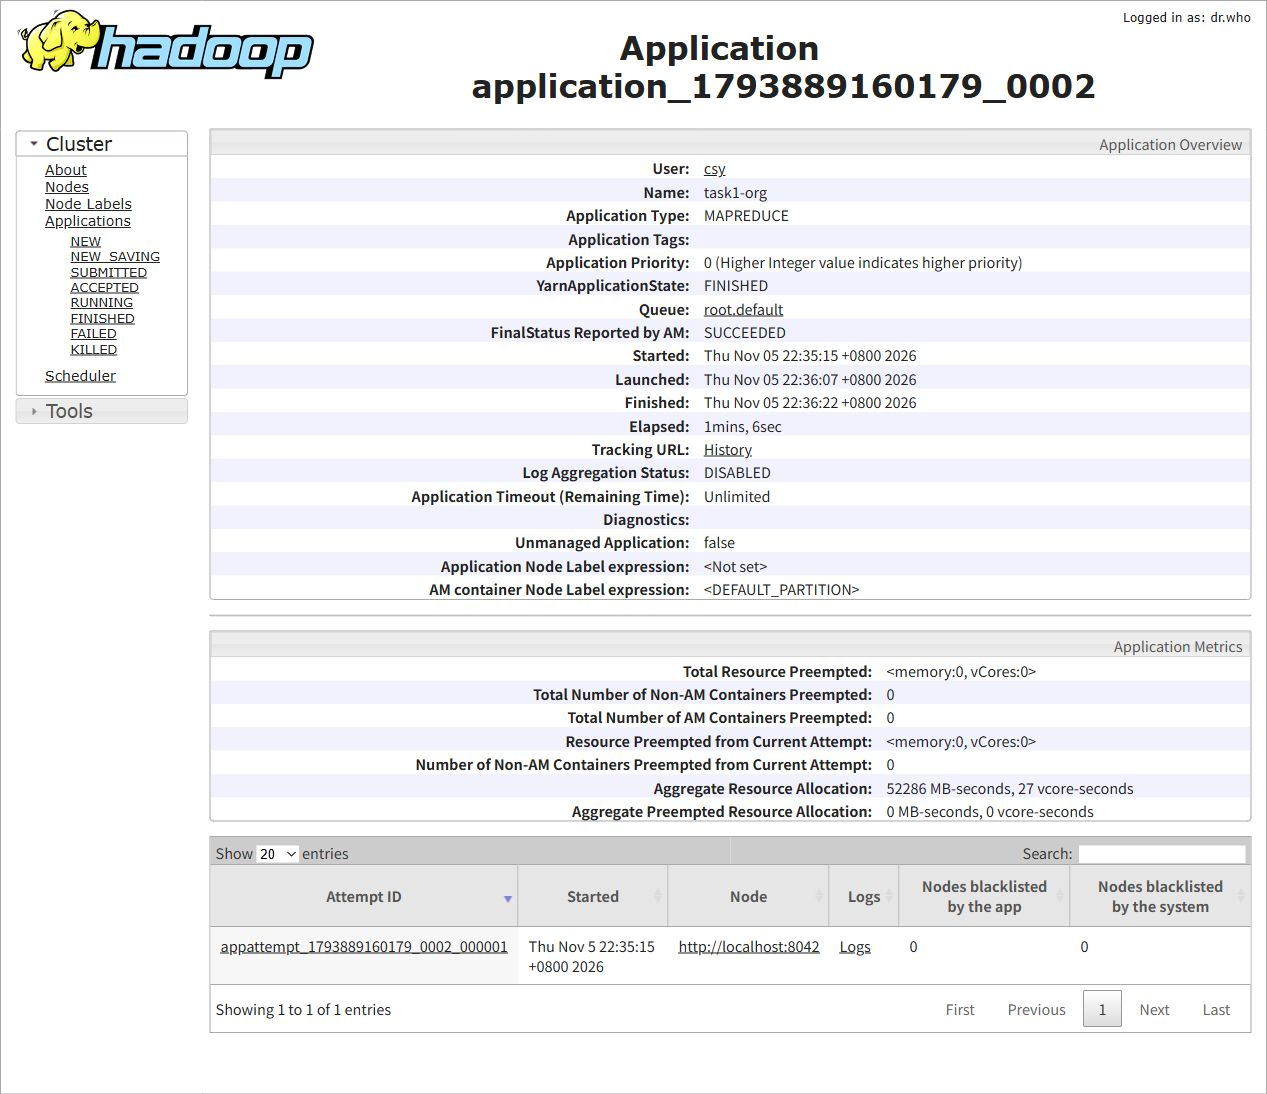
\includegraphics[width=\linewidth]{images/YARN作业成功详情.png}
\caption{YARN作业成功详情}
\end{figure}

\begin{figure}[H]\centering
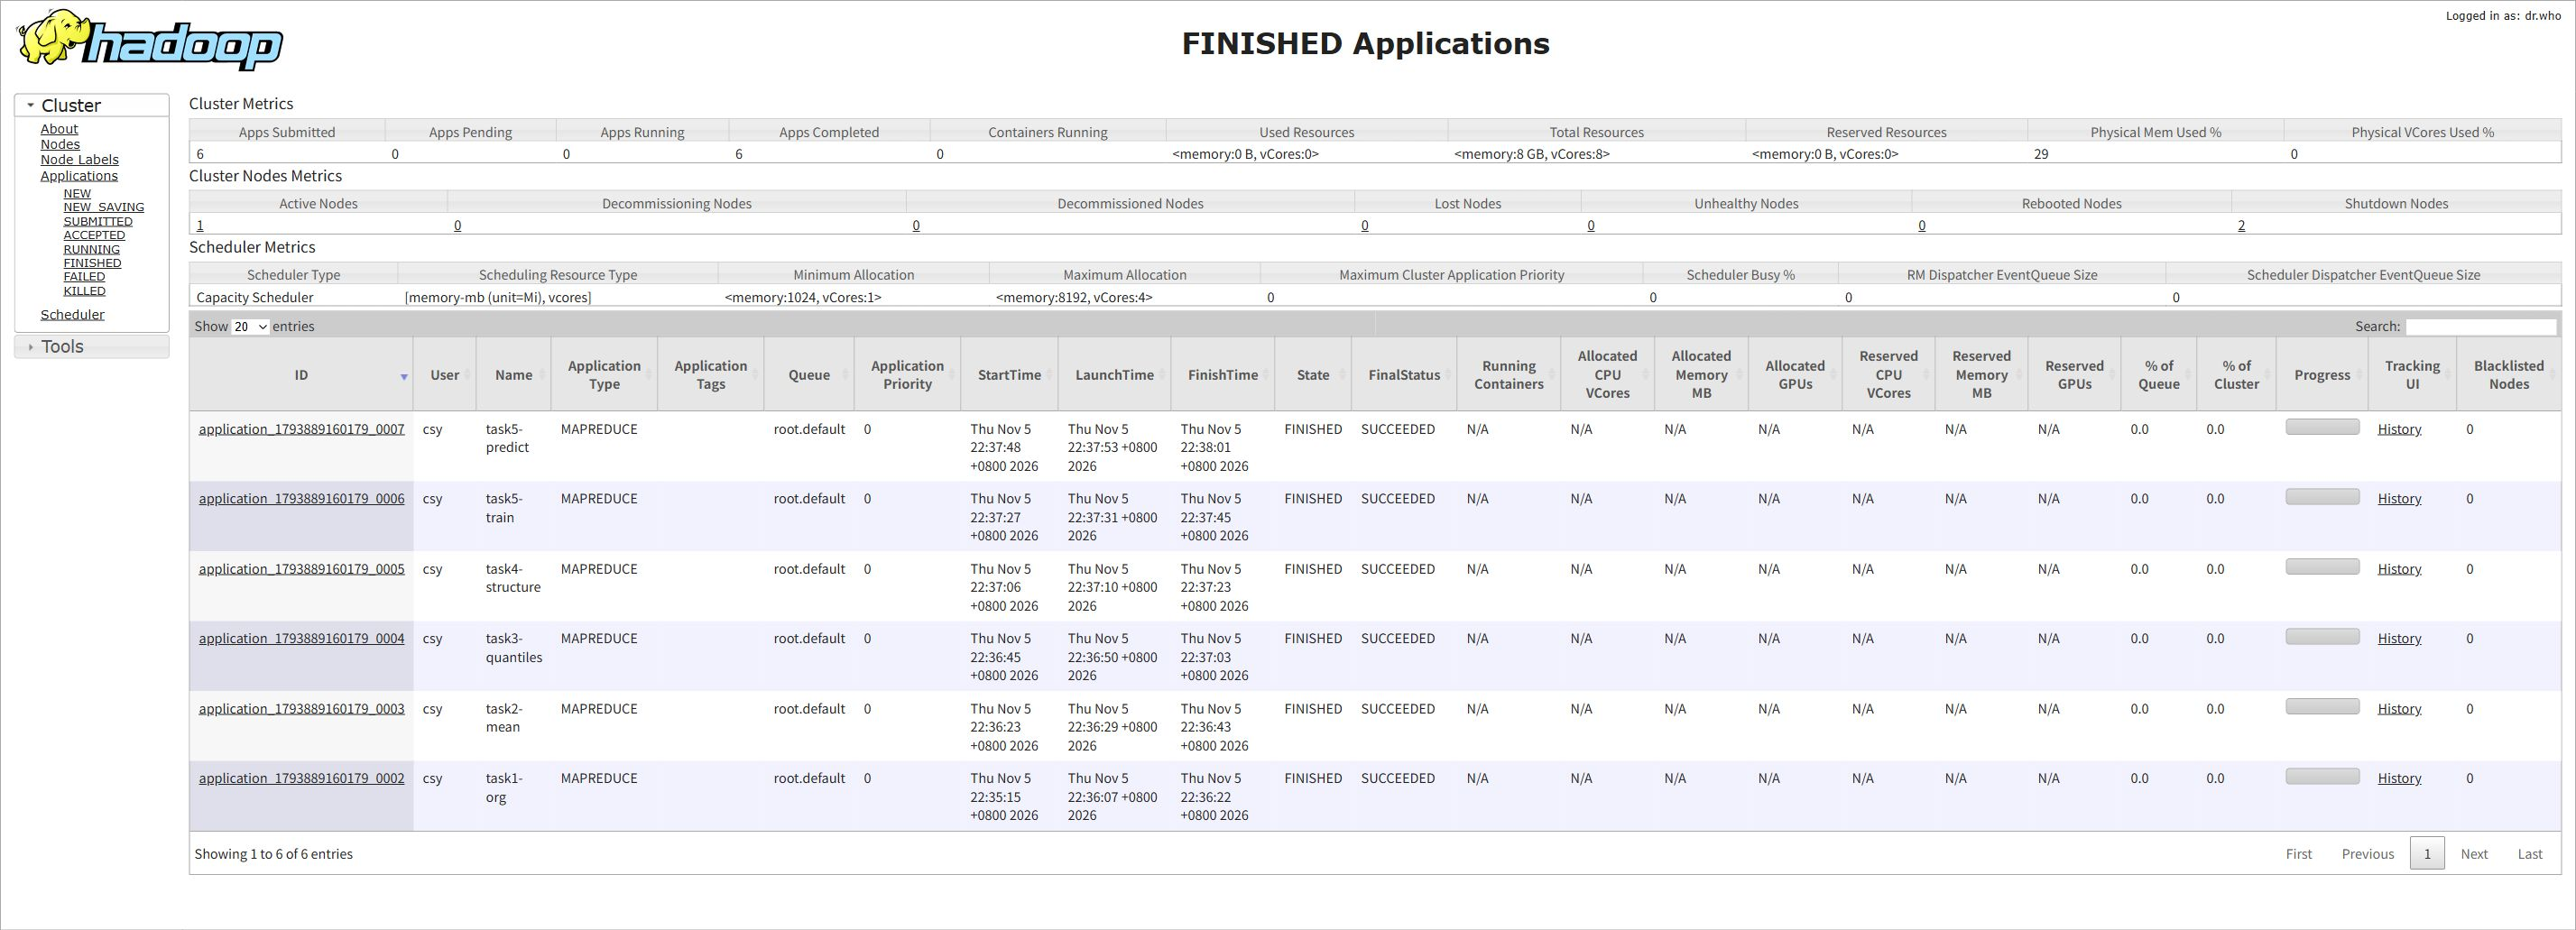
\includegraphics[width=\linewidth]{images/YARN全部作业成功总览.png}
\caption{YARN全部作业成功总览}
\end{figure}

\begin{figure}[H]\centering
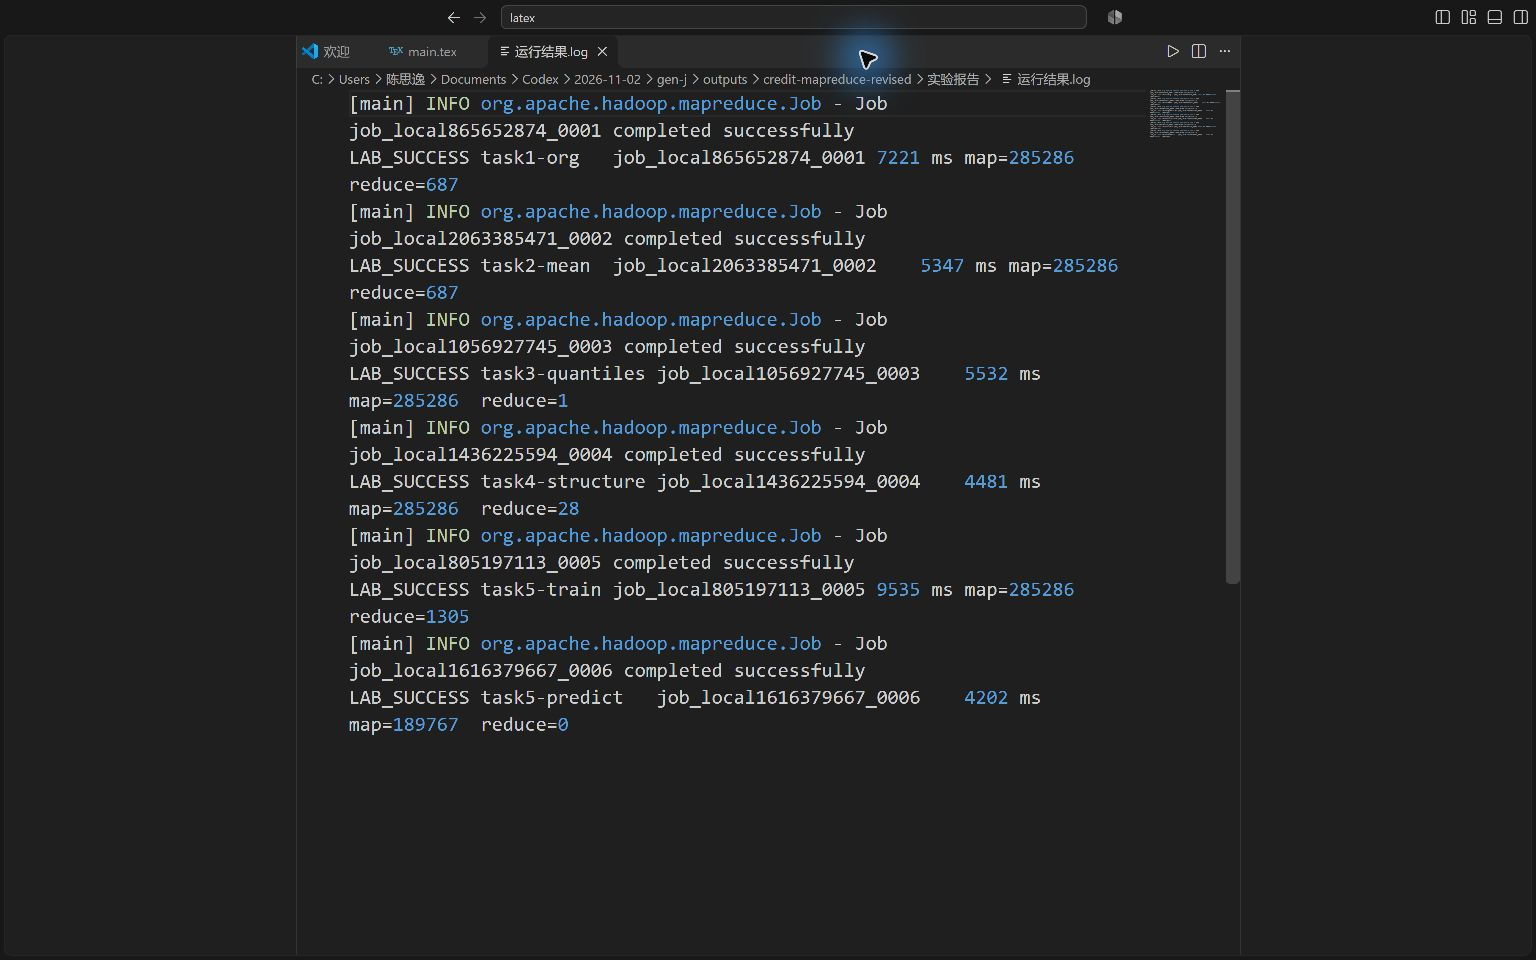
\includegraphics[width=\linewidth]{images/terminal.png}
\caption{编辑器查看实际运行日志的成功记录}
\end{figure}

任务 1、2 分别输出 687 行，任务 3 输出一行四分位数，任务 4 输出 28 行资产结构，模型计数文件输出 1,305 行，任务 5 输出 189,766 条预测。机构人数、资产负债合计、分位数和分层占比经独立计算核对一致。
\subsection{实验总结}
本实验将机构聚合、均值比较、资产排序和分类预测统一为键值转换与统计聚合问题。Combiner 降低了重复键的中间数据量，分布式缓存使每个 Mapper 能够访问机构统计或模型，作业依赖则保证下游使用一致的统计结果。

统计结果表明，客户资产分布存在明显差异，高资产层的理财及私人理财占比更高。预测模型在验证集上获得 0.6583 的 F1，但召回率为 50.87\%，后续可通过独立调参集选择代价敏感阈值，并增加时间外验证。工程上，单 Reducer 的全局排序适合本次数据规模；处理更大数据时可使用全序分区和分区计数定位全局秩，以降低排序瓶颈。
\end{document}
